\section{Normal Distribution/ Gaussian Distribution (${N}(\mu, \sigma^2)$, ${N}(x|\mu, \sigma^2)$)}


\begin{table}[H]
    \hfill
    \begin{minipage}{0.45\linewidth}
        \begin{figure}[H]
            \centering
            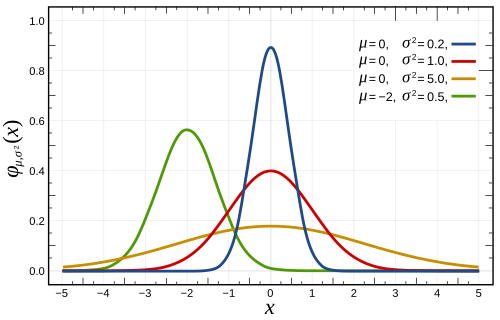
\includegraphics[
                width=\linewidth,
                height=5cm,
                keepaspectratio,
            ]{images/distributions/Normal_Distribution_PDF.svg.png}
            \caption{Normal Distribution: PDF \cite{wiki/Normal_distribution}}
        \end{figure}
    \end{minipage}
    \hfill
    \begin{minipage}{0.45\linewidth}
        \begin{figure}[H]
            \centering
            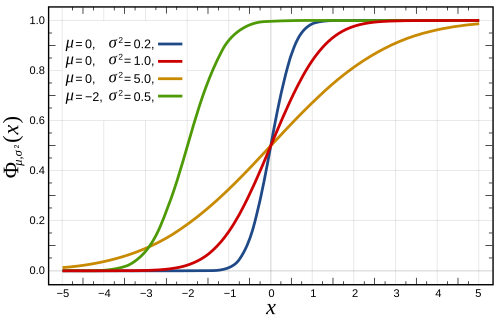
\includegraphics[
                width=\linewidth,
                height=5cm,
                keepaspectratio,
            ]{images/distributions/Normal_Distribution_CDF.svg.png}
            \caption{Normal Distribution: CDF \cite{wiki/Normal_distribution}}
        \end{figure}
    \end{minipage}
    \hfill
\end{table}

\begin{enumerate}
    \item Denoted by: $\mathcal{N}(\mu, \sigma^2)$
\end{enumerate}


\subsection{PDF ($f_{\mu, \sigma}(x)$ or $f(x|\mu, \sigma)$)}

\begin{enumerate}
    \item  $
        f_{\mu, \sigma}(x)
        = \dfrac{1}{\sigma\sqrt{2\pi}} \exp\dParenBrac{-\dfrac{(x-\mu)^2}{2\sigma^2}}
    $
    \hfill \cite{statistics/book/Statistics-for-Data-Scientists/Maurits-Kaptein}
    \begin{enumerate}
        \item[] $\mu \in \mbbR$: indicates the mean value of the population of the variable of interest
        \hfill \cite{statistics/book/Statistics-for-Data-Scientists/Maurits-Kaptein}

        \item[] $\sigma \in \mbbR$: indicates the standard deviation ($\sigma^2 > 0$)
        \hfill \cite{statistics/book/Statistics-for-Data-Scientists/Maurits-Kaptein}
    \end{enumerate}

    \item $f_{\mu, \sigma}(x) = \dfrac{1}{\sigma}\phi\dParenBrac{\dfrac{x-\mu}{\sigma}}$
    \hfill \cite{statistics/book/Statistics-for-Data-Scientists/Maurits-Kaptein}


    \item it can be used to approximate other PDFs when the sample size or the size of the data is getting large.
    \hfill \cite{statistics/book/Statistics-for-Data-Scientists/Maurits-Kaptein}

    \item This has the advantage that important features of the normal density function can be transferred to other densities when the approximation is quite close.
    \hfill \cite{statistics/book/Statistics-for-Data-Scientists/Maurits-Kaptein}

    \item The shape of the normal PDF is equal to the famous “bell-shape” curve
    \hfill \cite{statistics/book/Statistics-for-Data-Scientists/Maurits-Kaptein}

    \item areas under the curve:
    \begin{enumerate}
        \item $99.73\%$ of all the population values fall within the interval $[\mu - 3\sigma, \mu + 3\sigma]$
        \hfill \cite{statistics/book/Statistics-for-Data-Scientists/Maurits-Kaptein}

        \item $95.45\%$ of all the population values fall within the interval $[\mu - 2\sigma, \mu + 2\sigma]$ or
        \hfill \cite{statistics/book/Statistics-for-Data-Scientists/Maurits-Kaptein}
        \\
        $
            \dint_{\mu - 2\sigma}^{\mu + 2\sigma}
            \phi\dParenBrac{\dfrac{x-\mu}{\sigma}} dx
            =
            \dint_{-2}^{2}
            \phi(x) dx
            =
            0.9545
        $
        \hfill \cite{statistics/book/Statistics-for-Data-Scientists/Maurits-Kaptein}

        \item $95\%$ of the values fall within $[\mu - 1.96\sigma, \mu + 1.96\sigma]$
        \hfill \cite{statistics/book/Statistics-for-Data-Scientists/Maurits-Kaptein}
    \end{enumerate}

    \item  describes both positive and negative values
    \hfill \cite{statistics/book/Statistics-for-Data-Scientists/Maurits-Kaptein}

    \item a random measurement error that could be described by a normal PDF is more likely to be closer to zero than to be further away from zero (due to the bell shape of the density).
    \hfill \cite{statistics/book/Statistics-for-Data-Scientists/Maurits-Kaptein}
\end{enumerate}









\subsection{Maximum Likelihood}

\begin{enumerate}
    \item If our data set $\bm{x}$ is i.i.d., then we can therefore write the probability of the data set, given $\mu$  and $\sigma^2$, in the form
    \hfill \cite{ml/book/Pattern-Recognition-And-Machine-Learning/Christopher-M-Bishop}
    \\
    .\hfill
    $
        p(\bm{x}|\mu , \sigma^2)
        = \dprod^{N}_{n=1} \mathcal{N} (x_n|\mu , \sigma^2)
    $
    \hfill \cite{ml/book/Pattern-Recognition-And-Machine-Learning/Christopher-M-Bishop}

    \item Log likelihood function:
    \hfill \cite{ml/book/Pattern-Recognition-And-Machine-Learning/Christopher-M-Bishop}
    \\
    .\hfill
    $
        \ln (p (\bm{x}|\mu , \sigma ^2))
        = - \dfrac{1}{2\sigma ^2} \dsum^N_{n=1} (x_n - \mu )^2 - \dfrac{N }{2} \ln (\sigma ^2) - \dfrac{N }{2} \ln(2\pi)
    $
    \hfill \cite{ml/book/Pattern-Recognition-And-Machine-Learning/Christopher-M-Bishop}

    \item Maximizing $\ln (p (\bm{x}|\mu , \sigma ^2))$ with respect to $\mu$, we obtain the maximum likelihood solution given by
    $
        \mu_{ML}
        = \dfrac{1}{N} \dsum_{n=1}^N x_n
    $
    which is the sample mean, i.e., the mean of the observed values $\dCurlyBrac{x_n}$.
    \hfill \cite{ml/book/Pattern-Recognition-And-Machine-Learning/Christopher-M-Bishop}

    \item Maximizing $\ln (p (\bm{x}|\mu , \sigma ^2))$ with respect to $\sigma^2$, we obtain the maximum likelihood solution for the variance in the form
    $
        \sigma^2 _{ML} = \dfrac{1}{N} \dsum^N _{n=1} (x_n - \mu _{ML})^2
    $
    which is the sample variance measured with respect to the sample mean $\mu _{ML}$.
    \hfill \cite{ml/book/Pattern-Recognition-And-Machine-Learning/Christopher-M-Bishop}

    \item
    $\mbbE[\mu _{ML}] = \mu $
    \hfill
    $\mbbE[\sigma ^2_{ML}] = \dParenBrac{\dfrac{N - 1}{N}} \sigma ^2$
    \hfill \cite{ml/book/Pattern-Recognition-And-Machine-Learning/Christopher-M-Bishop}
\end{enumerate}







\subsection{Summary}

\begin{enumerate}

    \item
    \textbf{Notation}:
    $
        {\displaystyle {\mathcal {N}}(\mu ,\sigma ^{2})}
    $
    \hfill \cite{wiki/Normal_distribution}

    \item
    \textbf{Parameters}:
    \begin{enumerate}
        \item ${\displaystyle \mu \in \mathbb {R} }$ = mean (location)
        \hfill \cite{wiki/Normal_distribution}

        \item ${\displaystyle \sigma ^{2}\in \mathbb {R} _{>0}}$ = variance (squared scale)
        \hfill \cite{wiki/Normal_distribution}
    \end{enumerate}

    \item
    \textbf{Support/ Rand Var}:
    $x \in \mbbR$
    \hfill \cite{wiki/Normal_distribution}

    \item
    \textbf{PDF}:
    $ {\displaystyle {\dfrac {1}{\sqrt {2\pi \sigma ^{2}}}}e^{-{\dfrac {(x-\mu )^{2}}{2\sigma ^{2}}}}} $
    \hfill\cite{wiki/Normal_distribution}

    \item
    \textbf{CDF}:
    $ {\displaystyle \Phi \left({\dfrac {x-\mu }{\sigma }}\right)={\dfrac {1}{2}}\left[1+\operatorname {erf} \left({\dfrac {x-\mu }{\sigma {\sqrt {2}}}}\right)\right]} $
    \hfill\cite{wiki/Normal_distribution}

    \item
    \textbf{Quantile}:
    $ {\displaystyle \mu +\sigma {\sqrt {2}}\operatorname {erf} ^{-1}(2p-1)} $
    \hfill\cite{wiki/Normal_distribution}

    \item
    \textbf{Mean}:
    $ {\displaystyle \mu } $
    \hfill\cite{wiki/Normal_distribution}

    \item
    \textbf{Median}:
    $ {\displaystyle \mu } $
    \hfill\cite{wiki/Normal_distribution}

    \item
    \textbf{Mode}:
    $ {\displaystyle \mu } $
    \hfill\cite{wiki/Normal_distribution}

    \item
    \textbf{Variance}:
    $ {\displaystyle \sigma ^{2}} $
    \hfill\cite{wiki/Normal_distribution}

    \item
    \textbf{Precision}: $\beta = \dfrac{1}{\sigma^2}$
    \hfill \cite{ml/book/Pattern-Recognition-And-Machine-Learning/Christopher-M-Bishop}

    \item
    \textbf{Median absolute deviation (MAD)}:
    $ {\displaystyle \sigma {\sqrt {2}}\,\operatorname {erf} ^{-1}(1/2)} $
    \hfill\cite{wiki/Normal_distribution}

    \item
    \textbf{Average absolute deviation (AAD)}:
    $ {\textstyle \sigma {\sqrt {2/\pi }}} $
    \hfill\cite{wiki/Normal_distribution}

    \item
    \textbf{Skewness}: $0$
    \hfill\cite{wiki/Normal_distribution}

    \item
    \textbf{Excess kurtosis}: $0$
    \hfill\cite{wiki/Normal_distribution}

    \item
    \textbf{Entropy}: $ {\textstyle {\dfrac {1}{2}}\log(2\pi e\sigma ^{2})} $
    \hfill\cite{wiki/Normal_distribution}

    \item
    \textbf{Moment-generating function (MGF)}: $ {\displaystyle \exp(\mu t+\sigma ^{2}t^{2}/2)} $
    \hfill\cite{wiki/Normal_distribution}

    \item
    \textbf{Characteristic function (CF)}: $ {\displaystyle \exp(i\mu t-\sigma ^{2}t^{2}/2)} $
    \hfill\cite{wiki/Normal_distribution}

    \item
    \textbf{Fisher information}:
    \begin{enumerate}
        \item ${\displaystyle {\mathcal {I}}(\mu ,\sigma )={\begin{pmatrix}1/\sigma ^{2}&0\\0&2/\sigma ^{2}\end{pmatrix}}}$

        \item ${\displaystyle {\mathcal {I}}(\mu ,\sigma ^{2})={\begin{pmatrix}1/\sigma ^{2}&0\\0&1/(2\sigma ^{4})\end{pmatrix}}}$
    \end{enumerate}
    \hfill\cite{wiki/Normal_distribution}

    \item
    \textbf{Kullback–Leibler divergence}:
    ${\displaystyle D_{KL} = {1 \over 2}\left\{\left({\dfrac {\sigma _{0}}{\sigma _{1}}}\right)^{2}+{\dfrac {(\mu _{1}-\mu _{0})^{2}}{\sigma _{1}^{2}}}-1+\ln {\sigma _{1}^{2} \over \sigma _{0}^{2}}\right\}}$
    \hfill\cite{wiki/Normal_distribution}

    \item
    \textbf{Expected shortfall}:
    ${\displaystyle \mu +\sigma {\dfrac {{\dfrac {1}{\sqrt {2\pi }}}e^{\dfrac {-\left(q_{p}\left({\dfrac {X-\mu }{\sigma }}\right)\right)^{2}}{2}}}{1-p}}}$
    \hfill\cite{wiki/Normal_distribution}

    \item
    \textbf{second order moment}:
    $
        \mbbE[x^2]
        = \dint_{-\infty}^\infty \mathcal{N}(x|\mu, \sigma^2) x^2 dx
        = \mu^2 + \sigma^2
    $
    \hfill \cite{ml/book/Pattern-Recognition-And-Machine-Learning/Christopher-M-Bishop}

\end{enumerate}









\subsection{Normally Distributed Populations}

\begin{enumerate}
    \item we assume that the random variables $X_1 , X_2, \cdots , X_ n$ are i.i.d. normally distributed, $X _i \sim \mathcal{N} (\mu, \sigma^ 2)$
    \hfill \cite{statistics/book/Statistics-for-Data-Scientists/Maurits-Kaptein}

    \item \textbf{Properties}:
    \begin{enumerate}
        \item \textbf{Property 1}:
        \hfill \cite{statistics/book/Statistics-for-Data-Scientists/Maurits-Kaptein}
        \begin{enumerate}
            \item The sum of the random variables $\dsum^n _{i=1} X_ i$ is again \textbf{normally distributed}, but now with mean $n\mu$ and variance $n\sigma  ^2$ .
            \hfill \cite{statistics/book/Statistics-for-Data-Scientists/Maurits-Kaptein}

            \item Thus this implies that the sample average $\bar{X}$ has a normal distribution with mean $\mu$ and variance $\sigma ^ 2/n$ and thus has $\dfrac{\bar{X} - \mu}{\sigma /\sqrt{n}}$, a standard normal distribution function.
            \hfill \cite{statistics/book/Statistics-for-Data-Scientists/Maurits-Kaptein}
        \end{enumerate}

        \item \textbf{Property 2}:
        \begin{enumerate}
            \item The sum of the squared standardized random variables $\dfrac{1}{\sigma ^2} \dsum^n _{i=1} (X _i - \mu)^2$ is known to be \textbf{chi-square distributed} with $n$ degrees of freedom.
            \hfill \cite{statistics/book/Statistics-for-Data-Scientists/Maurits-Kaptein}

            \item The sum $\dfrac{1}{\sigma ^2} \dsum^n _{i=1} (X_ i - \bar{X} )^2$ is \textbf{chi-square distributed} with $n - 1$ degrees of freedom.
            \hfill \cite{statistics/book/Statistics-for-Data-Scientists/Maurits-Kaptein}
        \end{enumerate}

        \item \textbf{Property 3}:
        \begin{enumerate}
            \item Let $Z$ be standard normally distributed, $Z \sim \mathcal{N} (0, 1)$, let $V^ 2 _n$ be chi-square distributed with $n$ degrees of freedom, $V ^2 _n \sim \chi^2 _n$ , and assume that $Z$ and $V ^2 _n$ are independent.
            \hfill \cite{statistics/book/Statistics-for-Data-Scientists/Maurits-Kaptein}

            \item The distribution function of the ratio of this standard normal random variable and the square root of a chi-square $\dfrac{Z}{V_n /\sqrt{n}}$ has a so-called \textbf{Student t-distribution} with $n$ degrees of freedom. \hfill \cite{statistics/book/Statistics-for-Data-Scientists/Maurits-Kaptein}
        \end{enumerate}
    \end{enumerate}
\end{enumerate}


\subsubsection{Confidence Intervals for Normal Populations}

\begin{enumerate}
    \item $Z =\dfrac{\bar{X} - \mu}{\sigma/\sqrt{n}}$ is standard normal distributed
    \hfill (using property 1)
    \cite{statistics/book/Statistics-for-Data-Scientists/Maurits-Kaptein}

    \item $V ^2 _{n-1} = \dfrac{(n - 1)S^2}{\sigma^ 2} \sim \chi^2 _{n-1}$
    \hfill (using property 2)
    \cite{statistics/book/Statistics-for-Data-Scientists/Maurits-Kaptein}

    \item
    $
        \dfrac{\bar{X} - \mu }{S/\sqrt{n} }
        = \dfrac{( \bar{X} - \mu )/ (\sigma /\sqrt{n})}{\sqrt{(n - 1)S^2/\sigma ^ 2}/\sqrt{n - 1} }
        = \dfrac{Z}{V_{n-1}/\sqrt{n - 1} }
    $
    \hfill\cite{statistics/book/Statistics-for-Data-Scientists/Maurits-Kaptein}

    \item $\dfrac{\bar{X} - \mu }{S/\sqrt{n} }$ has a Student t-distribution with $n - 1$ degrees of freedom
    \hfill (using property 3)
    \cite{statistics/book/Statistics-for-Data-Scientists/Maurits-Kaptein}

    \item If $x _p ( f _t )$ is the $p$-th quantile of the Student t-distribution with $n - 1$ degrees of freedom, the $1 - 2 p$ confidence interval for $\mu$ (with $p < 0.5$) is now
    $
        \left (
            \bar{X} - x_{1- p} ( f _t ) \dfrac{S}{\sqrt{n}} ,
            \ \bar{X} + x_{1- p} ( f _t ) \dfrac{S}{\sqrt{n}}
        \right ]
    $
    \hfill\cite{statistics/book/Statistics-for-Data-Scientists/Maurits-Kaptein}

    \item Note that the only restriction on the sample size $n$, is that it should be larger than $2$, otherwise we cannot calculate a sample variance.
    \hfill\cite{statistics/book/Statistics-for-Data-Scientists/Maurits-Kaptein}

    \item When the sample size is increasing, the quantile of the Student t-distribution with $n - 1$ degrees of freedom converges to the quantile of the standard normal distribution.
    The quantiles of the t-distribution are already quite close to the same quantiles of the normal distribution when sample sizes are larger than $100$.
    \hfill\cite{statistics/book/Statistics-for-Data-Scientists/Maurits-Kaptein}

    \item The asymptotic $1 - 2 p$ confidence interval for the variance $\sigma^ 2$ is given by $(S^2 - z_{1- p} \hat{\tau}_n ,\ S^2 - z_{1- p} \hat{\tau}_n ]$, where  $\hat{\tau}_n = S^2\sqrt{\dfrac{b_2 + 2}{n}}$ and $b_2$ is the sample excess kurtosis.
    \hfill \cite{statistics/book/Statistics-for-Data-Scientists/Maurits-Kaptein}


    \item An alternative confidence interval for the variance $\sigma ^2$ can be created under the assumption that $X_1 , X_2, \cdots , X _n$ are i.i.d. normally distributed, $X_ i \sim \mathcal{N} (\mu, \sigma^ 2)$.
    Let $x _p ( f_{\chi^2} )$ be the $p$-th quantile of the chi-square distribution with $n - 1$ degrees of freedom.
    \hfill \cite{statistics/book/Statistics-for-Data-Scientists/Maurits-Kaptein}
    \begin{enumerate}
        \item Then $P(V ^2 _{n-1} \leq x _p ( f_{\chi^2} )) = p$.
        \hfill \cite{statistics/book/Statistics-for-Data-Scientists/Maurits-Kaptein}

        \item Then $P(\sigma ^ 2 \geq (n - 1)S^2/x _p ( f_{\chi ^2} )) = p$
        \hfill Using $\dParenBrac{V ^2 _{n-1} = \dfrac{(n - 1)S^2}{\sigma  ^2} \sim \chi ^2 _{n-1}}$
        \hfill \cite{statistics/book/Statistics-for-Data-Scientists/Maurits-Kaptein}

        \item
        $
            P(V^ 2 _{n-1} > x_{1- p} ( f_{\chi^2} )) = p
            \Longrightarrow
            P\dParenBrac{\sigma ^2 < \dfrac{(n - 1)S^2}{x_{1- p}( f_{\chi^2} )}} = p
        $
        \hfill \cite{statistics/book/Statistics-for-Data-Scientists/Maurits-Kaptein}

        \item Thus a $1 - 2 p$ confidence interval for the variance $\sigma^ 2$ is now given by
        $\left[\dfrac{(n - 1)S^2}{x_{1- p} ( f_{\chi^2} )}, \dfrac{(n - 1)S^2}{x _p ( f_{\chi^2})}  \right)$
        \hfill \cite{statistics/book/Statistics-for-Data-Scientists/Maurits-Kaptein}
    \end{enumerate}

    \item Confidence intervals for the population variance $\sigma^ 2$ immediately result in confidence intervals on the population standard deviation $\sigma$ by just taking the square root.
    \hfill \cite{statistics/book/Statistics-for-Data-Scientists/Maurits-Kaptein}
\end{enumerate}








\subsection{Distribution of the Sample Statistic ($T_n$)}

\subsubsection{Distribution of the Sample Average}

\begin{enumerate}
    \item let’s consider sample average $\bar{X} = \dfrac{1}{n} \dsum^n _{i=1} X_ i$ that tries to estimate the population mean $\mu( f )$.
    \hfill \cite{statistics/book/Statistics-for-Data-Scientists/Maurits-Kaptein}

    \item From central limit theorem, $X \sim \mathcal{N} \dParenBrac{\mu( f ),\ \dfrac{\sigma^ 2( f )}{n}}$ is approximately normally distributed.
    \hfill \cite{statistics/book/Statistics-for-Data-Scientists/Maurits-Kaptein}

    \item \textbf{Asymptotic Confidence Intervals}:
    \begin{enumerate}
        \item if $CI = 95\%$, and $CI = 1-2p$, $p=2.5\%$, $1-p = 97.5\%$ quantile of the standard normal distribution function is equal to $z_{1-p} = z_{0.975} = 1.96$
        \hfill \cite{statistics/book/Statistics-for-Data-Scientists/Maurits-Kaptein}

        \item Applying the $95\%$ asymptotic confidence interval for $\mu( f )$ using the estimator $\bar{X}$, results in
        \hfill \cite{statistics/book/Statistics-for-Data-Scientists/Maurits-Kaptein}
        \\[0.2cm]
        .\hfill
        $
            \left ( \bar{X} - \dfrac{1.96\ \sigma ( f )}{\sqrt{n}},
            \ \bar{X} + \dfrac{1.96\ \sigma ( f )}{\sqrt{n}} \right ]
        $
        \hfill \cite{statistics/book/Statistics-for-Data-Scientists/Maurits-Kaptein}

        \item Since the standard deviation $\sigma ( f )$ is unknown, we may replace $\sigma ( f )$ by an estimator.
        The most commonly used estimator is to use the sample standard deviation
        $S = \sqrt{\dfrac{1}{n - 1} \dsum^n _{i=1}(X_ i - \bar{X})^2}$.
        \hfill \cite{statistics/book/Statistics-for-Data-Scientists/Maurits-Kaptein}

        \item The $95\%$ confidence interval on $\mu( f )$ that can be calculated from the data is then equal to
        \hfill \cite{statistics/book/Statistics-for-Data-Scientists/Maurits-Kaptein}
        \\[0.2cm]
        .\hfill
        $
            \left ( \bar{X} - \dfrac{1.96\ S}{\sqrt{n}},
            \ \bar{X} + \dfrac{1.96\ S}{\sqrt{n}} \right ]
        $
        \hfill \cite{statistics/book/Statistics-for-Data-Scientists/Maurits-Kaptein}
    \end{enumerate}
\end{enumerate}








\subsection{Methods of Moments Estimation (MME)}

\begin{enumerate}
    \item The normal density has two parameters $\theta_1 = \mu$ and $\theta_2 = \sigma^ 2$.
    \hfill \cite{statistics/book/Statistics-for-Data-Scientists/Maurits-Kaptein}


\end{enumerate}


\subsection{Sums of Random Variables}

\begin{enumerate}
    \item Let $U$, $V$, and $W$ be three independent random variables and define $X = W + U$ and $Y = W + V$.
    When $U \sim \mathcal{N} (\mu_U , \sigma^2_U )$, $V \sim \mathcal{N} (\mu_V , \sigma^2_V )$, and $W \sim \mathcal{N} (\mu_W , \sigma^2_W )$, it can be shown that $X$ and $Y$ are bivariate normally distributed with
    \hfill \cite{statistics/book/Statistics-for-Data-Scientists/Maurits-Kaptein}
    \begin{multicols}{2}
    \begin{enumerate}
        \item $\mu _X = \mu _W + \mu _U$
        \hfill \cite{statistics/book/Statistics-for-Data-Scientists/Maurits-Kaptein}

        \item $\mu _Y = \mu _W + \mu _V$
        \hfill \cite{statistics/book/Statistics-for-Data-Scientists/Maurits-Kaptein}

        \item $\sigma ^2_X = \sigma ^2_W + \sigma ^2_U$
        \hfill \cite{statistics/book/Statistics-for-Data-Scientists/Maurits-Kaptein}

        \item $\sigma ^2_Y = \sigma ^2_W + \sigma ^2_V$
        \hfill \cite{statistics/book/Statistics-for-Data-Scientists/Maurits-Kaptein}

        \item $\rho = \dfrac{\sigma ^2_W }{\sqrt{(\sigma ^2_W + \sigma ^2_U )(\sigma ^2_W + \sigma ^2_V )}}$
        \hfill \cite{statistics/book/Statistics-for-Data-Scientists/Maurits-Kaptein}
    \end{enumerate}
    \end{multicols}
\end{enumerate}

















